\documentclass[11pt,a4paper,english]{article}
\usepackage{babel}
\usepackage{url}                      % for url
\usepackage{graphicx,subfigure,epsfig}% for figures
\usepackage[export]{adjustbox}        % for positioning figure e.g left
\usepackage{hyperref}                 % for hyperlink
\hypersetup{colorlinks=true,linkcolor=blue,filecolor=magenta, urlcolor=cyan}
\usepackage[backend=bibtex]{biblatex} % for bibliography
\usepackage{csquotes}                 % Recommended
\addbibresource{references.bib}       % separate by comma
\usepackage[nottoc]{tocbibind}        % to add references in the table of contents
\usepackage[usenames,dvipsnames,svgnames,table]{xcolor} % for color
\usepackage[pagecolor=none]{pagecolor}% color for the page
\usepackage{afterpage}                % color for afterpage
\usepackage[ampersand]{easylist}      % for listing


% Creating Title
\title{Inserting images in Latex}
\author{Bhishan Poudel}
\date{Wed Apr 20, 2016}
% Begin document
\begin{document}
\maketitle
\tableofcontents
\listoffigures
\clearpage

\section{List using package easylist}

\begin{easylist}[enumerate]

& Level 1.
  && Level 2.
    &&& Level 3.
      &&&& Level 4.
        &&&&& Level 5.   
\end{easylist}

\section{Inserting images in Latex}
%%%%%%%%%%%%%%%%%%%% figure environment start %%%%%%%%%%%%%%%%%%%%%%%%%%%%%%
\begin{figure}[ht!]
\centering
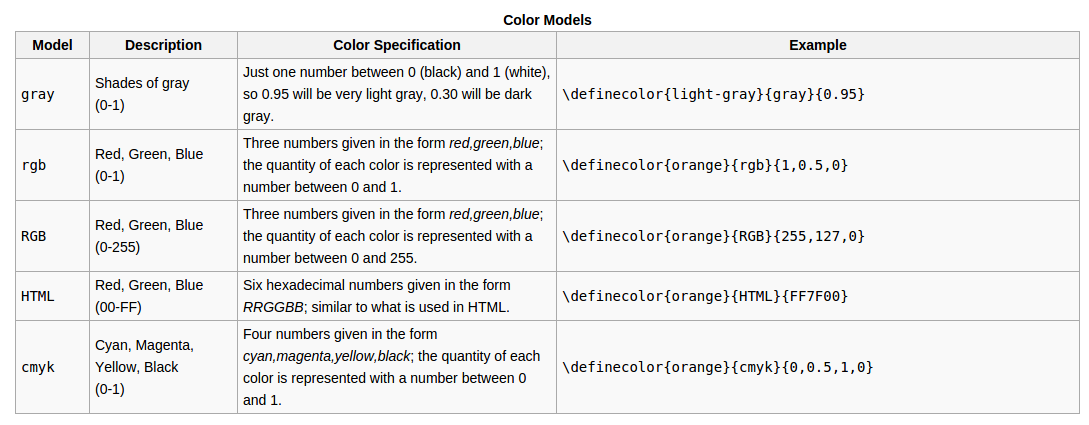
\includegraphics[scale=0.3]{images/color_modes.png}
\caption{color modes}
\label{fig:color_modes}   
\end{figure}
%%%%%%%%%%%%%%%%%%%% figure environment start %%%%%%%%%%%%%%%%%%%%%%%%%%%%%%
\begin{figure}[ht!]
\centering
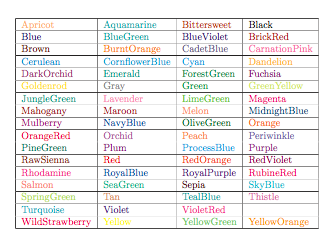
\includegraphics[scale=1.0]{images/default_colors.png}
\caption{default colors}
\label{fig:default_colors}   
\end{figure}
%%%%%%%%%%%%%%%%%%%% figure environment start %%%%%%%%%%%%%%%%%%%%%%%%%%%%%%
\begin{figure}[ht!]
\centering
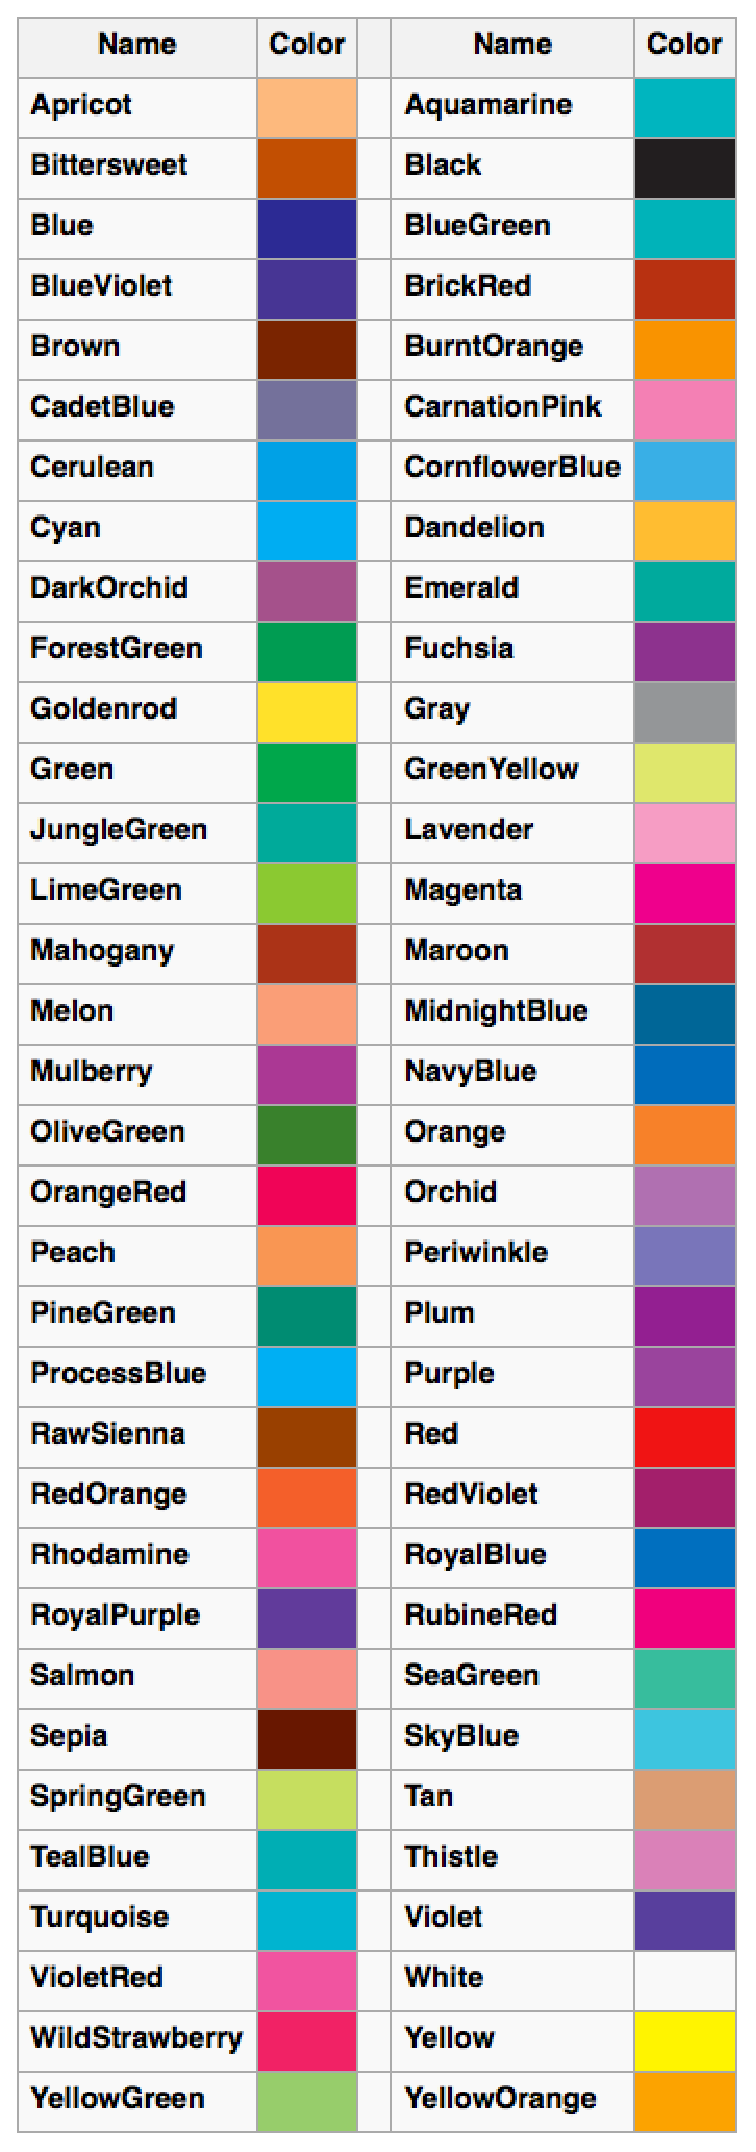
\includegraphics[scale=0.5]{images/dvips_colors.eps}
\caption{dvips colors}
\label{fig:dvips_colors}   
\end{figure}
%%%%%%%%%%%%%%%%%%%% figure environment start %%%%%%%%%%%%%%%%%%%%%%%%%%%%%%
\begin{figure}[ht!]
\centering
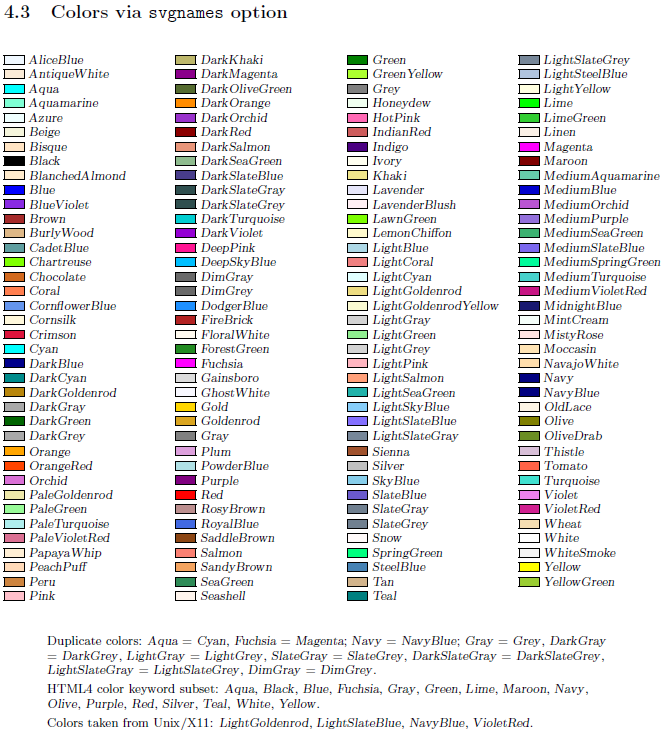
\includegraphics[scale=0.9]{images/svgnames_with_duplicates.png}
\caption{svgnames with duplicates}
\label{fig:svgnames_with_duplicates}   
\end{figure}
\clearpage

%%%%%%%%%%%%%%%%%%%% figure environment end %%%%%%%%%%%%%%%%%%%%%%%%%%%%%%%

\section{colors in Latex}
The initialization of additional commands like usenames allows you to use 
names of the default colors, the same 16 base colors as used in HTML. 
The dvipsnames allows you access to more colors, another 64, and svgnames 
allows access to about 150 colors. The initialization of "table" allows 
colors to be added to tables by placing the color command just before the table. 
The package loaded here is the xcolor package.

If you need more colors, then you may also want to look at adding the x11names 
to the initialization section as well, this offers more than 300 colors, 
but you need to make sure your xcolor package is the most recent you can download.


The predefined color names are

black, blue, brown, cyan, darkgray, gray, green, lightgray, 
lime, magenta, olive, orange, 
pink, purple, red, teal, violet, white, yellow.\\

\pagecolor{LightGoldenrod} % \afterpage{\pagecolor{none}} % afterpage does not work
\emph{some black text, \color{blue} followed by a blue fragment}, going black again.
{\color[rgb]{1,0,0} This text will appear red-colored}
\textcolor[rgb]{0,1,0}{This text will appear green-colored}
\textcolor[rgb]{0.1,0.40,0.03}{This text will appear custom}

The 68 standard colors known to dvips

Invoke the package with the usenames and dvipsnames option. 
If you are using tikz or pstricks package you must declare the xcolor 
package before that, otherwise it will not work.
\indent This is indented text

\end{document}

